%---%
\chapter{Áttekintés}
%---%

\section{A kvantumkommunikáció napjainkig}

A kvantumkommunikációról valamint kvantuminformatikáról mint kutatási területről, valamikor a 90-es évek eleje-közepe óta beszélhetünk, habár az általa vizsgált és használt főbb jelenségekkel a fizika már az 1920-as években is foglalkozott. Elég csak azt tekinteni, hogy a kvantummechanika egyik mai meghatározó alapköve az 1926-ban publikált Schrödinger-egyenlet \cite{schrodinger1926undulatory}. Az azóta eltelt időben a témához kapcsolható talán leghíresebb történés az 1980-as évekig az 1935-ös ún. EPR-paradoxon \cite{einstein1935can} valamint ennek kapcsán Bell 1964-es válasza \cite{bellt1964einstein}. Az EPR-paradoxonban Einsteinék összefonódott párok azon különleges tulajdonságát vizsgálták, hogy az egyik részecskén elvégzett véletlen eredményű mérés, hatással van az összefonódott pár másik tagjára is, távolságtól függetlenül.  Mivel az azonnali információterjedés lehetősége a relativitáselméletben megismertekkel ellenkezik, helyi rejtett, számunkra ismeretlen változók ötletével álltak elő ennek magyarázatára. Így ezekbe az ismeretlen változókba lehetséges lehetne előre eltárolni információt, ami alapján a számunkra véletlennek tűnő méréseknél a pár mégis korreláló eredményeket mutathat. Mivel a kvantummechanikában ilyen rejtett változók nincsenek, ezért szerintük a kvantummechanikának hiányosnak kellett lennie. Bell 1964-es írásában erre reflektál. Az általa levezetett egyenlőtlenség lehetővé tette ezen elméletek kísérleti tesztelését, melyek később a kvantummechanika jóslatait igazolták, a rejtett változós elképzeléssel szemben.\\
 Az 1980-as években már kezdték vizsgálni ezen jelenségek későbbi lehetséges alkalmazásait, 1982-ben született a később meghatározó ``No Cloning Theorem'' \cite{wootters1982single}, ami a tetszőleges kvantumbit másolhatatlanságát mondja ki, továbbá 1984-ben merült fel az első kvantumkriptográfia protokoll ötlete is \cite{BB84}. Az 1990-es évektől kezdődően pedig kísérleti megvalósításokkal is találkozhatunk. További meghatározó eljárások születtek, mint például a kvantum teleportációs protokoll \cite{bennett1993teleporting}, majd ennek későbbi kísérleti megvalósítása \cite{bouwmeester1997experimental}, vagy akár az elméletben RSA titkosítás törésére is használható Shor-algoritmus \cite{shor1999polynomial}. Kvantumkommunikációs szempontból 1992-ben először hajtottak végre sikerrel kvantum kulcsszétosztást \cite{bennett1992experimental}, valamint 1993-ban felmerült az összefonódás megosztás ötlete \cite{zukowski1993event}, amit 1998-ban kísérletileg is megvalósítottak \cite{pan1998experimental}. Fontos előrelépés volt még az első összefonódás tisztító eljárások \cite{bennett1996purification}\cite{deutsch1996quantum} megjelenése is, később ezen újítások segítségével vázolták fel a kvantum ismétlő ötletét \cite{briegel1998quantum}. \\
 Az elkövetkezendő években egyre hatékonyabb eljárások, valamint az új technológiák segítségével pontosabb és megbízhatóbb kísérletek készültek. Ezt bizonyítja, hogy a 2000-es évek közepétől kezdtek elérhetővé válni (főleg kvantumkriptográfiában) a nagyközönség számára is használható kvantumos termékek. A folyamatos fejlődés megfigyelhető a kapcsolódó kutatások növekedésén is, idővel egyre több helyen alakultak a témába vágó kutatóközpontok, valamint kísérleti kvantumhálózatok. Egyre közeledünk az előzetes kutatások iparban való felhasználhatóságához. Ezt mutatják a közelmúltban a témában elért eredmények is. Ezek közül az egyik talán legjelentősebb a kínaiak által 2016-ben Föld körüli pályára állított műhold \cite{chinasat} kvantum kulcsszétosztás tesztelésére, melyről már kísérleti eredmények is származnak \cite{yin2017satellite}. Megemlítendő még, hogy felismerve a területben rejlő lehetőségeket, a kvantumos kutatások támogatása bekerült az Európai Unió fejlesztési tervébe is, amely keretében 1 milliárd euró értékben támogatnak kvantumtechnológiai kutatásokat és fejlesztéseket \cite{manifesto}.\\
 \begin{figure}[h]
\centering
\makebox[\textwidth][c]{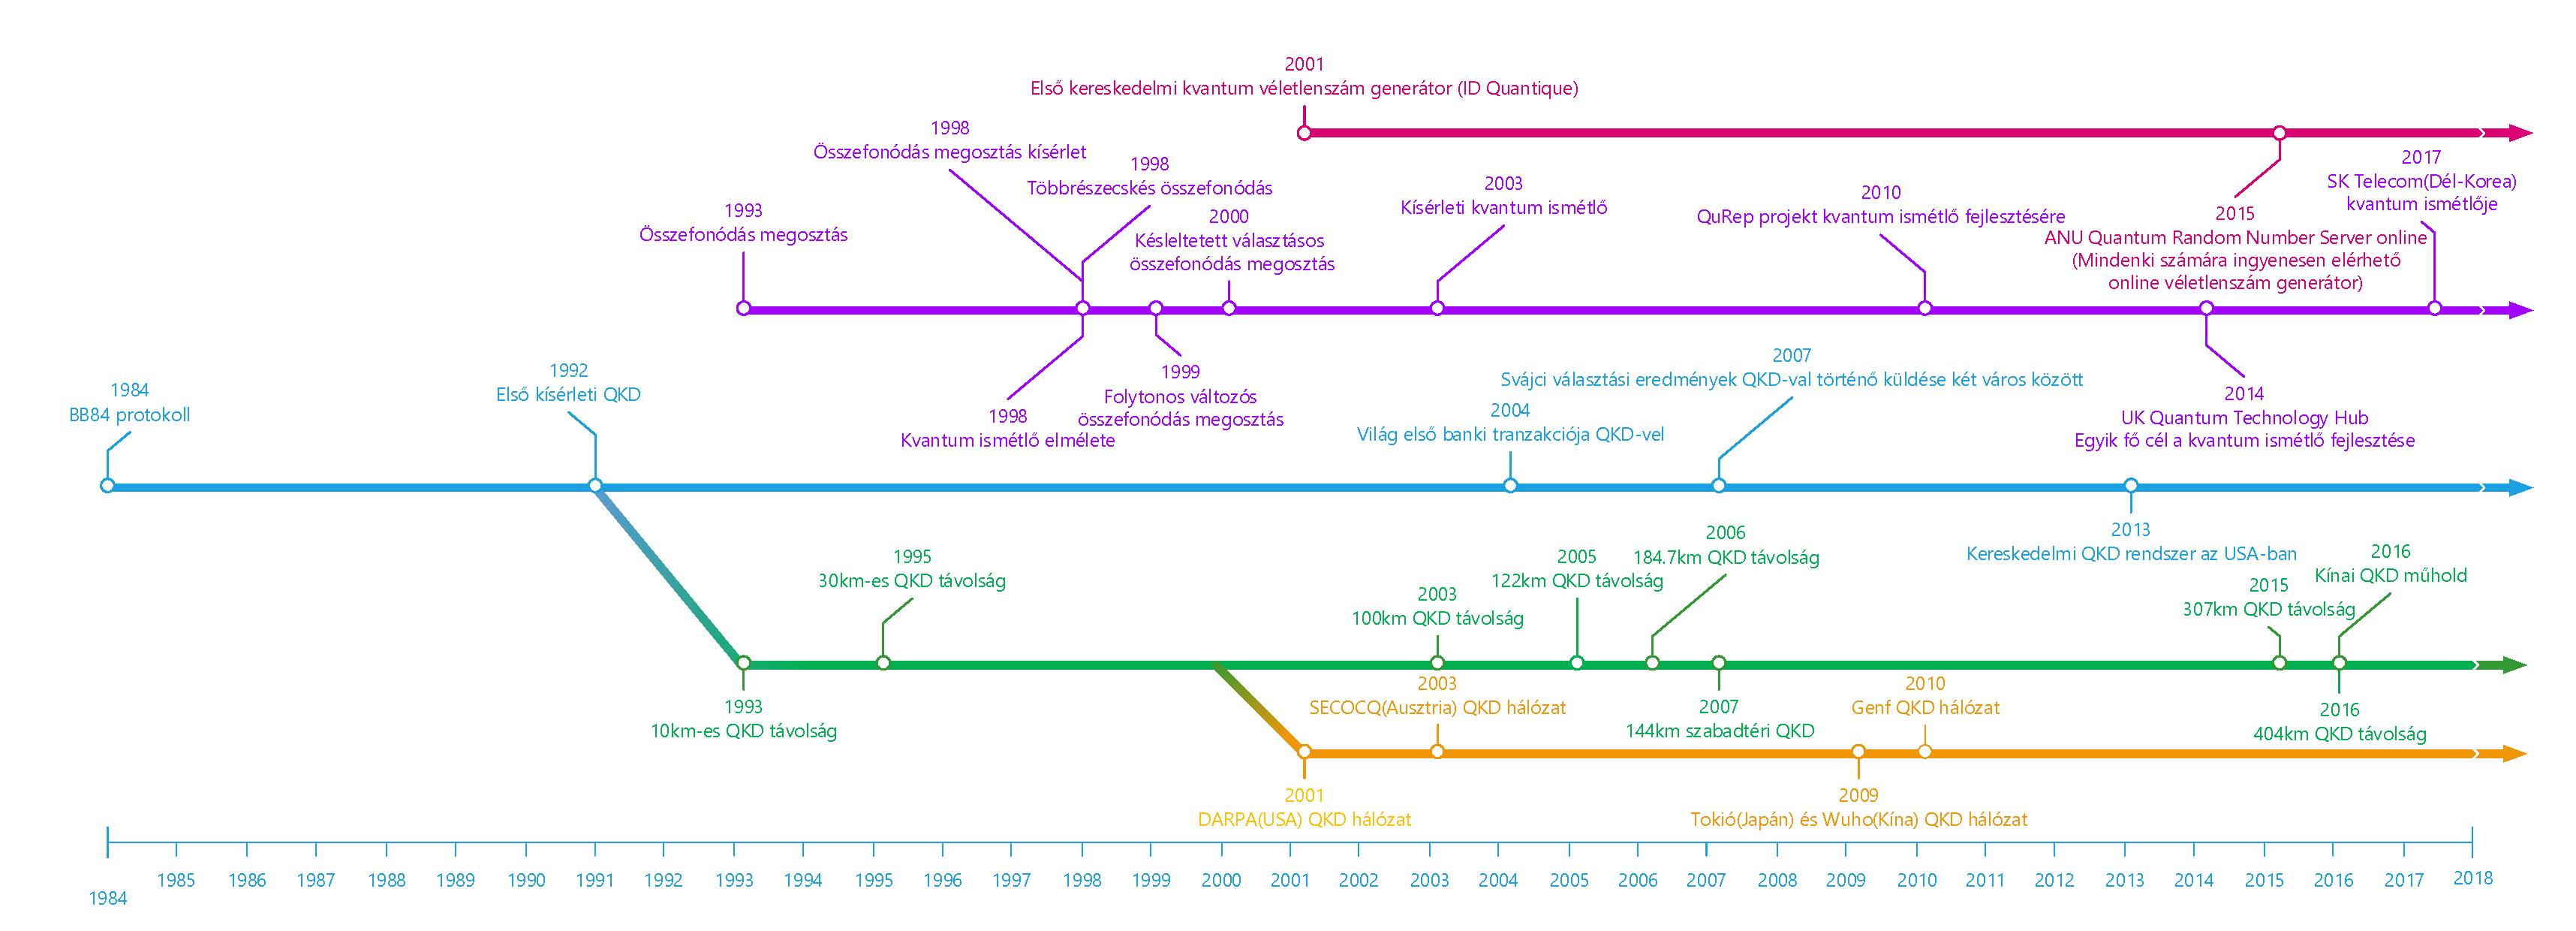
\includegraphics[height=\textheight]{timeline}}
\caption[Kvantumkommunikáció timeline]{Kvantumkommunikáció fejlődése 1984-től}
\end{figure}
A ``kvantum internet'' \cite{kimble2008quantum}\cite{pirandola2016unite} megvalósításához azonban még mindig le kell küzdeni a hozzáférési pontok közti távolságból adódó problémákat. Habár a kapcsolódó technológiák fokozatosan javultak az évek során, olyan megbízható, hibatűrő rendszer ami ehhez kéne még nincs. A közeljövőben erre két kutatási terület is kínálhat megoldást: egyes kvantum hibajavító kódok \cite{lidar2013quantum} melyek alkalmazhatóak hálózatokra is \cite{zhang2013quantum}, valamint a kvantum ismétlők\cite{uphoff2016integrated}\cite{krovi2016practical}\cite{pfister2016quantum}\cite{li2016heralded}. A dolgozat a továbbiakban ezek közül a kvantum ismétlőkkel foglalkozik. 



